\documentclass{article}
\usepackage{graphicx} % Required for inserting images
\usepackage[ngerman]{babel}
\usepackage{enumitem}
\usepackage{float}
\usepackage{chngcntr}
\usepackage{glossaries}
\usepackage{tabularx}
\counterwithin{figure}{section}
\counterwithin{table}{section}
\setlength\parindent{0pt}

\makeglossaries

\newglossaryentry{Attributsableitung}
{
    name=Attributsableitung,
    description={Platzhalter-Implementierung eines Glossar-Eintrags}
}

\newglossaryentry{Verkehrsmodell}
{
    name=Verkehrsmodell,
    description={Platzhalter-Implementierung eines Glossar-Eintrags}
}

\newglossaryentry{Discrete Choice}
{
    name=Discrete Choice,
    description={Platzhalter-Implementierung eines Glossar-Eintrags}
}

\newglossaryentry{Projektdatei}
{
    name=Projektdatei,
    description={Enthält eine CSV-Datei, sowie eventuell Attributsableitungen, Alternativen und vorherige Ergebnisse.}
}

\newglossaryentry{Valide Attributsableitung}
{
    name=Valide Attributsableitung,
    description={Eine Attributsableitung, die syntaktisch korrekt ist und dessen Referenzen auf Attribute alle existieren.}
}

\newglossaryentry{Invalide Attributsableitung}
{
    name=Valide Attributsableitung,
    description={Eine Attributsableitung, die syntaktisch inkorrekt ist oder die eine Referenz auf ein nicht-existierendes Attribut hat.}
}

\newglossaryentry{Valide Alternative}
{
    name=Valide Alternative,
    description={Eine Alternative, dessen Name eindeutig ist, dessen Nutzenfunktion syntaktisch korrekt ist und dessen Referenzen auf Attribute alle existieren.}
}

\newglossaryentry{Invalide Alternative}
{
    name=Invalide Alternative,
    description={Eine Alternative, dessen Name bereits vorkommt, dessen Nutzenfunktion syntaktisch inkorrekt ist oder die eine Referenz auf ein nicht-existierendes Attribut hat.}
}

\newglossaryentry{Alternative}
{
    name=Alternative,
    description={Ein alternatives Verkehrsmittel.}
}

\newacronym{Ableitung}{Ableitung}{Attributsableitung}

\newacronym{WK}{WK}{Wunschkriterium}

\newacronym{CSV}{CSV}{Comma-separated values}

\title{Pflichtenheft \\ \large Einflussfaktoren auf die Verkehrsmittelwahl\\ -- Baukasten für Discrete Choice Modelle}
\author{Kevin Boehnke \\ \texttt{uxpkw@student.kit.edu}
\and Floriane Bresser \\ \texttt{uspvq@student.kit.edu}
\and Damian Reich \\ \texttt{uqppn@student.kit.edu}
\and Alissa Saleh \\ \texttt{unmbc@student.kit.edu}
\and Michael Schur \\ \texttt{ufkmz@student.kit.edu}}
\date{24. Mai 2023}

\begin{document}
\clearpage\maketitle\thispagestyle{empty}
\newpage
\clearpage\tableofcontents\thispagestyle{empty}
\newpage
\pagenumbering{arabic}

\section{Einleitung}

Im Alltag wirken sich viele Einflüsse auf die Verkehrsmittelwahl aus: Die demographische Entwicklung, Infrastrukturmaßnahmen, Veränderungen in den Siedlungsstrukturen, Steuerungsmaßnahmen, veränderte Energiepreise oder Maßnahmen des Mobility Pricings sind nur ein Teil dieser Faktoren. Um eine quantitative Basis zu schaffen, die verkehrsplanerische, betriebswirtschaftliche und politische Entscheidungen unterstützt, werden Verkehrsmodelle eingesetzt.\newline

Ein Modell zur Analyse unterschiedlicher Faktoren auf die Verkehrsnachfrage ist die Discrete-Choice Modellierung. Hier werden jeder Verkehrsalternative Wahrscheinlichkeiten anhand von Nutzenfunktionen zugewiesen, die von unbekannten Parametern abhängen. Diese Parameter werden mittels der Maximum-Likelihood-Methode aus Umfrageergebnissen geschätzt, in denen die Befragten Aussagen über ihr Verhalten bei der Verkehrsmittelwahl machen. Ebenfalls können Parameter mittels der Stated Choice Methode geschätzt werden. Diese basiert auf hypothetischen Entscheidungssituationen zwischen Alternativen. Hierbei bestehen die Alternativen, zwischen denen sich die Befragten entscheiden müssen, aus unterschiedlichen Attributen. %Eine Stated Choice Parameterschätzung beginnt mit Entscheidungen über die Alternativen und ihrer Attribute und der Erwartung möglicher Nutzenfunktionen zur Optimierung des Designs des Stated Choice Experiment. Anschließend wird das Design implementiert und die Befragung umgesetzt. Im letzten Schritt soll das Aufbereiten der Daten und Abschätzen der Parameter erfolgen.
\newline

Der entwickelte Baukasten übernimmt das Einlesen und Aufbereiten der Erhebungsdaten und ermöglicht, durch Berechnungen im Rahmen der Discrete-Choice Modellierung, eine Schätzung und Visualisierung der Parameter für die Verkehrsalternativen. Durch die Möglichkeit, individuelle Nutzenfunktionen und Attributsableitungen zu definieren, soll das Produkt diesen Ablauf vereinfachen und eine automatisierte Parameterschätzung mit Signifikanzen sowie die Visualisierung der Ergebnisse des Modells ermöglichen. 

\subsection{Anmerkungen}
Wunschkriterien außerhalb des Blocks \textbf{Zielbestimmung} werden durch (\textit{WK}) markiert.

\clearpage
\section{Zielbestimmung}
Das Produkt unterstützt Verkehrsingenieure dabei, Discrete-Choice Modelle in der Verkehrsmittelwahl zu erstellen, modifizieren und visualisieren.
\subsection{Musskriterien}
\begin{itemize}
    \item[\textbf{/MK10/}] Der Nutzer kann Erhebungsdaten im CSV-Format importieren.
    \item[\textbf{/MK20/}] Der Nutzer kann Attributsableitungen hinzufügen, ändern, und löschen.
    \newline Folgende Möglichkeiten stehen dem Nutzer zur Verfügung:
    \begin{itemize}[leftmargin=.7in]
        \item[\textbf{/MK21/}] Intervalle
        \item[\textbf{/MK22/}] Gruppen
        \item[\textbf{/MK23/}] Logische Ausdrücke
        \item[\textbf{/MK24/}] Vergleiche
    \end{itemize}
    \item[\textbf{/MK30/}] Der Nutzer kann Alternativen hinzufügen, ändern und löschen.
    \item[\textbf{/MK35/}] Der Nutzer kann für jede Alternative eine Nutzenfunktion definieren und ändern.
    \begin{itemize}[leftmargin=.7in]
        \item[\textbf{/MK36/}] Der Nutzer kann Linearkombinationen für die Nutzenfunktion verwenden.
    \end{itemize}
    \item[\textbf{/MK40/}] Der Nutzer kann Alternativen exportieren und importieren.
    \item[\textbf{/MK50/}] Der Nutzer kann die Parameter und Signifikanz aus gegebener Eingabe und Modellstruktur berechnen lassen.
    \item[\textbf{/MK60/}] Das Programm bietet eine Schnittstelle für andere Bibliotheken zur Parameterschätzung und Signifikanzgewinnung. 
    \begin{itemize}
        \item Es wird standardmäßig das Python Paket \textit{Biogeme} verwendet.
    \end{itemize}
    \item[\textbf{/MK70/}] Das Programm visualisiert die gewonnenen Parameter und Signifikanzniveaus.
    \item[\textbf{/MK80/}] Der Nutzer kann die Ergebnisse der Berechnung und die Visualisierung exportieren.
    \item[\textbf{/MK90/}] Der Nutzer kann die Tabelle im CSV-Format mit den Attributsableitungen exportieren.
    \item[\textbf{/MK100/}] Das Programm bietet eine Schnittstelle um die Parameteraufteilung zu erweitern oder einzuteilen anhand der Signifikanzniveaus.
    \item[\textbf{/MK110/}] Der Nutzer kann ein Projekt als Projektdatei speichern und laden.
\end{itemize}

\subsection{Wunschkriterien}
\begin{itemize}
    \item[\textbf{/WK10/}] Das Programm unterstützt arbiträre Funktionen für Attributsableitungen.
    \item[\textbf{/WK20/}] Der Nutzer kann die importierte CSV-Datei graphisch darstellen lassen.
    \item[\textbf{/WK30/}] Der Nutzer wird durch weitere Funktionen in der Bedienbarkeit unterstützt. \newline Folgende Funktionen können dem Nutzer helfen:
    \begin{itemize}[leftmargin=.7in]
        \item[\textbf{/WK31/}] Autovervollständigung
        \item[\textbf{/WK32/}] Typhinweise
        \item[\textbf{/WK33/}] Fehlerunterbindung
    \end{itemize}
    \item[\textbf{/WK40/}] Die Nutzenfunktionen können verschachtelt werden.
    \newline Folgende Möglichkeiten stehen dem Nutzer zur Verfügung:
    \begin{itemize}[leftmargin=.7in]
        \item[\textbf{/WK41/}] Arithmetik: $\beta \cdot (T + (\beta_2 \cdot X_2 \cdots))$
        \item[\textbf{/WK42/}] Exponentialfunktionen: $\log(T)$, ${\rm e}^T$
        \item[\textbf{/WK43/}] Potenzen: $\beta \cdot X^3$
    \end{itemize}
    \item[\textbf{/WK50/}] Das Programm kann um andere Modell-Strukturen erweitert werden.
    \begin{itemize}
        \item Beispielsweise um das \textit{Nested Logit Model}
    \end{itemize}
    \item[\textbf{/WK60/}] Der Nutzer kann die Schwellwerte für die Signifikanz in der Visualisierung konfigurieren.
    \begin{itemize}
        \item Beispielsweise im \textit{Apollo Package}:\newline $|T-Ratio | > 1.95$, $|Robust T-Ratio | > 1.95$
    \end{itemize}    
    \item[\textbf{/WK70/}] Das Programm bietet einen vollwertigen Algorithmus zur Bestimmung von Signifikanzgruppen und Aufteilungen.
    \item[\textbf{/WK80/}] Export Interface 
\end{itemize}

%\subsection{Abgrenzungskriterien}

\clearpage
\section{Produkteinsatz}
\subsection{Anwendungsbereiche}
Der vorgesehene Anwendungsbereich ist die Verkehrsmodellierung aus Befragungsdaten im Bereich der Verkehrswissenschaften. Die Anwendung eignet sich zur Modellierung für eine Prognose als Basis für verkehrsplanerische, betriebswirtschaftliche und politische Entscheidungen. Ebenso kann sie Verwendung in der Recherche finden.

\subsection{Zielgruppen}
Das Produkt richtet sich an Verkehrsingenieure und Verkehrswissenschaftler. Zur Verwendung sind keine besonderen Vorkenntnisse im technischen Bereich notwendig.\newline 
Es wird eine Open Source Veröffentlichung angestrebt.
  
\subsection{Betriebsbedingungen}
Der Baukasten wird als Desktopanwendung konzipiert, die in Büroumgebung ausgeführt wird. Übliche Betriebsbedingungen sind die Nutzung zu konventionellen Arbeitszeiten. Es ist keine Beobachtung während der Ausführung notwendig, unbeaufsichtigter Betrieb wird unterstützt und die Ausführung kann unterbrochen und zu späteren Zeitpunkten fortgeführt werden. Zur Ausführung der Anwendung wird keine Internetverbindung benötigt.
Mindestanforderungen für die Ausführung der Anwendung ist ein Laptop mit 8 GB RAM, i5 (4 Kerne, 8 logische Kerne) und Betriebssystem Windows 10 oder Windows 11. Ebenfalls soll die Anwendung auf der Workstation mit Windows Server, 8 Kerne (16 logische Kerne) ausgeführt werden können (\textit{WK}).

\clearpage
\section{Produktumgebung}
\subsection{Software}
\begin{itemize}
    \item Die Software wird in Python geschrieben.
    \item Betriebssystem: Windows 10 oder Windows 11
    \item Die Software wird als Open Source veröffentlicht und erweiterbar sein.
\end{itemize}
\subsection{Hardware}
\begin{itemize}
    \item Das Produkt ist eine Desktopanwendung.
    \begin{itemize}
        \item Mindestanforderung: Laptop, 8 GB RAM, Intel Core i5 (4 Kerne, 8 logische Kerne)
        \item (\textit{WK})\textit{: Workstation, Windows Server, 8 Kerne (16 logische Kerne)}
    \end{itemize}
\end{itemize}
\subsection{Schnittstelle}
\begin{itemize}
    \item Die Software nimmt Dateien im CSV-Format entgegen.
    \item Die Anwendung soll über eine Schnittstelle andere Bibliotheken zur Parameterschätzung einbinden können.
    \begin{itemize}
        \item beispielsweise das \textit{Apollo Package}
    \end{itemize}
\end{itemize}

\clearpage
\section{Produktfunktionen}
\subsection{Diagramm}
Das Anwendungsfalldiagramm für alle Produktfunktionen des Programms:
\begin{figure}[H]%
  \centering
  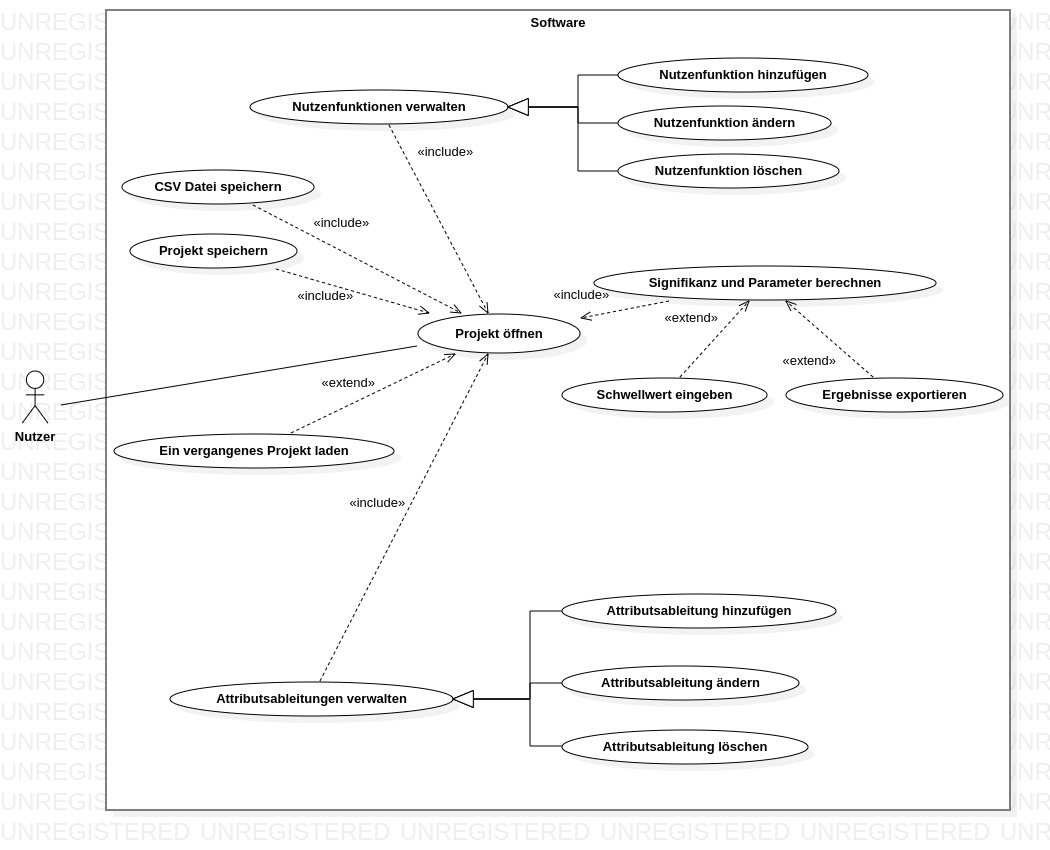
\includegraphics[width=15cm]{specifications/img/use-case/UseCaseDiagram6.jpg}
  \caption{Anwendungsfalldiagramm}
\end{figure} 
\newpage
\subsection{Funktionsübersicht}
Hier eine Übersicht aller Produktfunktionen: \\
[0.05in]
\textbf{/F10/} Neues Projekt erstellen \\
\textbf{/F11/} Projekt laden \\
\textbf{/F12/} Projekt speichern \\
\textbf{/F13/} CSV-Datei exportieren \\
\textbf{/F15/} Attributsableitung hinzufügen \\
\textbf{/F16/} Attributsableitung ändern \\
\textbf{/F17/} Attributsableitung löschen \\
\textbf{/F20/} Alternative hinzufügen \\
\textbf{/F21/} Alternative ändern \\
\textbf{/F22/} Alternative löschen \\
\textbf{/F25/} Berechnung durchführen \\
\textbf{/F28/} Ergebnisse exportieren \\
\textbf{/F30/} Schwellwerte konfigurieren
%\newpage
\\[0.2in]
\subsection{Funktionsbeschreibungen}
\subsubsection*{/F10/ Neues Projekt erstellen}
\begin{itemize}
    \item[\underline{Ziel:}] Ein neues Projekt erstellen, in das eine bereits existierende CSV-Datei mit den Erhebungsdaten importiert wird.
    \item[\underline{Vorbedingung:}] keine
    \item[\underline{Beschreibung:}]
    \begin{enumerate}
        \item Nutzer wählt die CSV-Datei aus.
        \item Nutzer speichert gegebenenfalls offenes Projekt.
    \end{enumerate}
    \item[\underline{Erweiterung:}]
    \begin{itemize}
        \item[2a.] Nutzer bricht den Vorgang ab.
    \end{itemize}
    \item[\underline{Kriterien:}] /MK10/
\end{itemize}

\subsubsection*{/F11/ Projekt laden}
\begin{itemize}
    \item[\underline{Ziel:}] Ein existierendes Projekt öffnen.
    \item[\underline{Vorbedingung:}] keine
    \item[\underline{Beschreibung:}]
    \begin{enumerate}
        \item Nutzer wählt die Projektdatei aus.
        \item Nutzer speichert gegebenenfalls offenes Projekt.
    \end{enumerate}
    \item[\underline{Erweiterung:}]
    \begin{itemize}
        \item[2a.] Nutzer bricht den Vorgang ab.
    \end{itemize}
    \item[\underline{Kriterien:}] /MK110/
\end{itemize}

\subsubsection*{/F12/ Projekt speichern}
\begin{itemize}
    \item[\underline{Ziel:}] Benutzerdefinierte Attributsableitungen, Nutzenfunktionen, Ergebnisse aus durchgeführten Berechnungen und die originale CSV-Datei sollen in einer Projektdatei gespeichert werden.
    \item[\underline{Vorbedingung:}] Projekt ist geöffnet.
    \item[\underline{Beschreibung:}] 
    \begin{enumerate}
        \item Nutzer speichert das Projekt.
    \end{enumerate}
    \item[\underline{Erweiterung:}]
    \begin{itemize}
        \item[1a.] Nutzer wählt den Speicherort, falls das Projekt zuvor noch nicht gespeichert wurde.
    \end{itemize}
    \item[\underline{Kriterien:}] /MK110/
\end{itemize}

\subsubsection*{/F13/ CSV-Datei exportieren}
\begin{itemize}
    \item[\underline{Ziel:}] Die originale CSV-Datei mit hinzugefügten und berechneten Spalten der definierten Attributsableitungen in neuer CSV-Datei exportieren.
    \item[\underline{Vorbedingung:}] Projekt ist geöffnet.
    \item[\underline{Beschreibung:}] 
    \begin{enumerate}
        \item Nutzer exportiert die CSV-Datei.
        \item Nutzer wählt den Speicherort.
    \end{enumerate}
    \item[\underline{Kriterien:}] /MK90/
\end{itemize}

\subsubsection*{/F15/ Attributsableitung hinzufügen}
\begin{itemize}
    \item[\underline{Ziel:}] Neue Attributsableitung definieren und hinzufügen. 
    \item[\underline{Vorbedingung:}] Projekt ist geöffnet.
    \item[\underline{Beschreibung:}]
    \begin{enumerate}
        \item Nutzer will neue Attributsableitung hinzufügen.
        \item Nutzer gibt die Attributsableitung ein.
    \end{enumerate}
    \item[\underline{Erweiterung:}]
    \begin{itemize}
        \item[2a.] Beinhaltet die Attributsableitung einen Syntax- oder Typfehler, wird sie nicht angenommen und eine Fehlermeldung weist darauf hin.
    \end{itemize}
    \item[\underline{Kriterien:}] /MK20/; /MK21/; /MK22/; /MK23/; /MK24/;\newline/WK10/; /WK30/; /WK31/; /WK32/; /WK33/
\end{itemize}

\subsubsection*{/F16/ Attributsableitung ändern}
\begin{itemize}
    \item[\underline{Ziel:}] Existierende Attributsableitung ändern.
    \item[\underline{Vorbedingung:}] Projekt ist geöffnet. Attributsableitung existiert.
    \item[\underline{Beschreibung:}]
    \begin{enumerate}
        \item Nutzer wählt die Attributsableitung aus.
        \item Nutzer ändert die vorherige Attributsableitung.
    \end{enumerate}
    \item[\underline{Erweiterung:}]
    \begin{itemize}
        \item[2a.] Beinhaltet die neue Attributsableitung einen Syntax- oder Typfehler, wird sie nicht angenommen und eine Fehlermeldung weist darauf hin.
    \end{itemize}
    \item[\underline{Kriterien:}] /MK20/; /MK21/; /MK22/; /MK23/; /MK24/;\newline/WK10/; /WK30/; /WK31/; /WK32/; /WK33/
\end{itemize}

\subsubsection*{/F17/ Attributsableitungen löschen}
\begin{itemize}
    \item[\underline{Ziel:}] Existierende Attributsableitung löschen.
    \item[\underline{Vorbedingung:}] Projekt ist geöffnet. Attributsableitung existiert.
    \item[\underline{Beschreibung:}]
    \begin{enumerate}
        \item Nutzer löscht die Funktion.
    \end{enumerate}
    \item[\underline{Erweiterung:}]
    \begin{itemize}
        \item[1a.] Wird die Attributsableitung in einer anderen Attributsableitung oder Nutzenfunktion referenziert, weist eine Warnung darauf hin. Der Nutzer kann anschließend fortfahren oder abbrechen.
    \end{itemize}
    \item[\underline{Kriterien:}] /MK20/
\end{itemize}

\subsubsection*{/F20/ Alternative hinzufügen}
\begin{itemize}
    \item[\underline{Ziel:}] Neue Nutzenfunktion definieren und hinzufügen.
    \item[\underline{Vorbedingung:}] Projekt ist geöffnet.
    \item[\underline{Beschreibung:}]
    \begin{enumerate}
        \item Nutzer will neue Nutzenfunktion hinzufügen.
        \item Nutzer gibt den Namen der Alternative ein.
        \item Nutzer gibt die Nutzenfunktion ein.
    \end{enumerate}
    \item[\underline{Erweiterung:}]
    \begin{itemize}
        \item[2a.] Besitzt eine andere Alternative bereits den Namen, weist eine Fehlermeldung darauf hin. Der Name kann anschließend geändert werden.
        \item[3a.] Beinhaltet die Nutzenfunktion einen Syntax- oder Typfehler, wird sie nicht angenommen und eine Fehlermeldung weist darauf hin.
    \end{itemize}
    \item[\underline{Kriterien:}] /MK30/; /MK35/; /MK36/; /WK30/; /WK31/; /WK32/; /WK33/
\end{itemize}

\subsubsection*{/F21/ Alternative ändern}
\begin{itemize}
    \item[\underline{Ziel:}] Existierende Alternative ändern.
    \item[\underline{Vorbedingung:}] Projekt ist geöffnet. 
    \item[\underline{Beschreibung:}]
    \begin{enumerate}
        \item Nutzer wählt die Alternative aus.
        \item Nutzer ändert die vorherige Alternative.
    \end{enumerate}
    \item[\underline{Erweiterung:}]
    \begin{itemize}
        \item[2a.] Besitzt eine andere Alternative bereits den Namen, weist eine Fehlermeldung darauf hin. Der Name kann anschließend geändert werden.
        \item[2b.] Beinhaltet die Nutzenfunktion einen Syntax- oder Typfehler, wird sie nicht angenommen und eine Fehlermeldung weist darauf hin.
    \end{itemize}
    \item[\underline{Kriterien:}] /MK30/; /MK35/; /MK36/; /WK30/; /WK31/; /WK32/; /WK33/
\end{itemize}

\subsubsection*{/F22/ Alternative löschen}
\begin{itemize}
    \item[\underline{Ziel:}] Existierende Alternative löschen.
    \item[\underline{Vorbedingung:}] Projekt ist geöffnet. Alternative existiert.
    \item[\underline{Beschreibung:}]
    \begin{enumerate}
        \item Nutzer löscht die Alternative.
    \end{enumerate}
    \item[\underline{Kriterien:}] /MK30/
\end{itemize}

\subsubsection*{/F25/ Berechnung durchführen}
\begin{itemize}
    \item[\underline{Ziel:}] Parameter und zugehörige Signifikanzen berechnen lassen und visualisieren.
    \item[\underline{Vorbedingung:}] Projekt ist geöffnet. Es existiert mindestens eine Alternative.
    \item[\underline{Beschreibung:}]
    \begin{enumerate}
        \item Mindestens eine Alternative existiert.
        \item Nutzer lässt die Berechnung durchführen.
        \item Nach der Berechnung werden die Ergebnisse visualisiert.
    \end{enumerate}
    \item[\underline{Kriterien:}] /MK50/; /MK60/; /MK70/ 
\end{itemize} 

\subsubsection*{/F28/ Ergebnisse exportieren}
\begin{itemize}
    \item[\underline{Ziel:}] Ergebnisse der Parameter- und Signifikanz-Berechnung exportieren.
    \item[\underline{Vorbedingung:}] Projekt ist geöffnet. Berechnung wurde durchgeführt.
    \item[\underline{Beschreibung:}]
    \begin{enumerate}
        \item Berechnung wird durchgeführt.
        \item Nutzer exportiert die Ergebnisse in einer CSV-Datei.
        \item Nutzer wählt den Speicherort.
    \end{enumerate}
    \item[\underline{Kriterien:}] /MK80/
\end{itemize}

\subsubsection*{/F30/ Schwellwerte konfigurieren}
\begin{itemize}
    \item[\underline{Ziel:}] Schwellwerte in der Visualisierung der Ergebnisse ändern.
    \item[\underline{Vorbedingung:}] Projekt ist geöffnet. Berechnung wurde durchgeführt.
    \item[\underline{Beschreibung:}]
    \begin{enumerate}
        \item Berechnung wird durchgeführt.
        \item Nutzer ändert den Schwellwert.
    \end{enumerate}
    \item[\underline{Kriterien:}] /WK60/
\end{itemize}

\clearpage
\section{Produktdaten}
Die Speicherung der Daten erfolgt ausschließlich lokal.
\subsection{Projektdaten}
Bei der Speicherung eines Projekts wird ein projektabhängiger Ordner erstellt, falls keiner vorhanden ist. Die folgenden Daten werden in dem Ordner angelegt oder überschrieben. \newline
/D20/ und /D30/ werden regelmäßig automatisch gespeichert, falls sie bereits als Datei im Projekt-Ordner vorhanden sind.
\subsubsection*{/D10/ Erhebungsdaten}
Die CSV-Datei, die dem Projekt zugrunde liegt, wird unverändert gespeichert.
\subsubsection*{/D11/ Attributsableitungen}
Die benutzerdefinierten Attributsableitungen werden als Funktionen in einer JSON-Datei gespeichert.
\subsubsection*{/D12/ Alternativen und Nutzenfunktionen}
Die benutzerdefinierten Alternativen mit jeweiliger Nutzenfunktion werden in einer JSON-Datei gespeichert.
\subsubsection*{/D13/ Parameter und Signifikanzen}
Berechnete Parameter mit jeweiliger Signifikanz werden in einer CSV-Datei gespeichert.
%\subsubsection*{/D70/ CSV-Datei mit Berechnungen}
%Die vollständige CSV-Datei, die sowohl Rohdaten als auch Attribute enthält wird temporär gespeichert.
\subsection{Funktionen}
\subsubsection*{/D20/ Alternativen und Nutzenfunktionen}
Die benutzerdefinierten Alternativen mit jeweiliger Nutzenfunktion können seperat vom Projekt gespeichert werden. Diese können anschließend in andere Projekte geladen werden.


\clearpage
\section{Produktleistungen}
\subsection{Benutzbarkeit}
\begin{itemize}
    \item[\textbf{/LB10/}] Die Berechnung der Ergebnisse kann jederzeit abgebrochen werden.
\end{itemize}
\subsection{Zuverlässigkeit}
\begin{itemize}
    \item[\textbf{/LF10/}] Die Daten /D20/ und /D30/ werden regelmäßig automatisch gespeichert, falls sie bereits als Datei im Projekt-Ordner vorhanden sind.
\end{itemize}
\subsection{Kommunikation}
\begin{itemize}
    \item[\textbf{/LK10/}] Das Laden einer korrupten CSV- oder Projektdatei wird mit einer Fehlermeldung abgebrochen. Das Programm wird dadurch nicht beeinträchtigt.
    \item[\textbf{/LK20/}] Ungültige Nutzenfunktionen werden visuell und mit Fehlermeldung markiert.
    \item[\textbf{/LK30/}] Ungültige Attributsableitungen werden visuell und mit Fehlermeldung markiert.
    \item[\textbf{/LK40/}] Das Speichern einer Projektdatei mit ungültigen Nutzenfunktionen oder ungültigen Attributsableitungen wird dem Nutzer mit einer Fehlermeldung angemerkt. Danach kann der Nutzer den Speichervorgang fortführen oder abbrechen.
    \item[\textbf{/LK50/}] Das Laden einer Projektdatei mit ungültigen Nutzenfunktionen oder ungültigen Attributsableitungen wird dem Nutzer mit einer Fehlermeldung angemerkt.
    \item[\textbf{/LK60/}] Das Exportieren einer CSV-Datei bei Existenz von ungültigen Attributsableitungen wird dem Nutzer mit einer Fehlermeldung angemerkt. Danach kann der Nutzer den Vorgang fortführen oder abbrechen.
\end{itemize}
\subsection{Effizienz}
\begin{itemize}
    \item[\textbf{/LE10/}] Das Importieren einer CSV-Datei ($\leq$ 500MB) erfolgt innerhalb von maximal 5 Sekunden.
    \item[\textbf{/LE20/}] Das Laden einer Projektdatei ($\leq$ 500MB CSV-Datei, $\leq$ 20 Alternativen, $\leq$ 30 Attributsableitungen) erfolgt innerhalb von maximal 10 Sekunden.
    \item[\textbf{/LE30/}] Die Berechnung der Ergebnisse und die Visualisierung erfolgt innerhalb von maximal 10 Sekunden.
    \item[\textbf{/LE40/}] Das Exportieren der Ergebnisse und der Visualisierung erfolgt innerhalb von maximal 5 Sekunden.
    \item[\textbf{/LE50/}] Das Exportieren der CSV-Datei mit den Attributsableitungen erfolgt innerhalb von maximal 3 Sekunden.
\end{itemize}

\clearpage
\section{Benutzerschnittstelle}
\begin{figure}[H]%
  \centering
  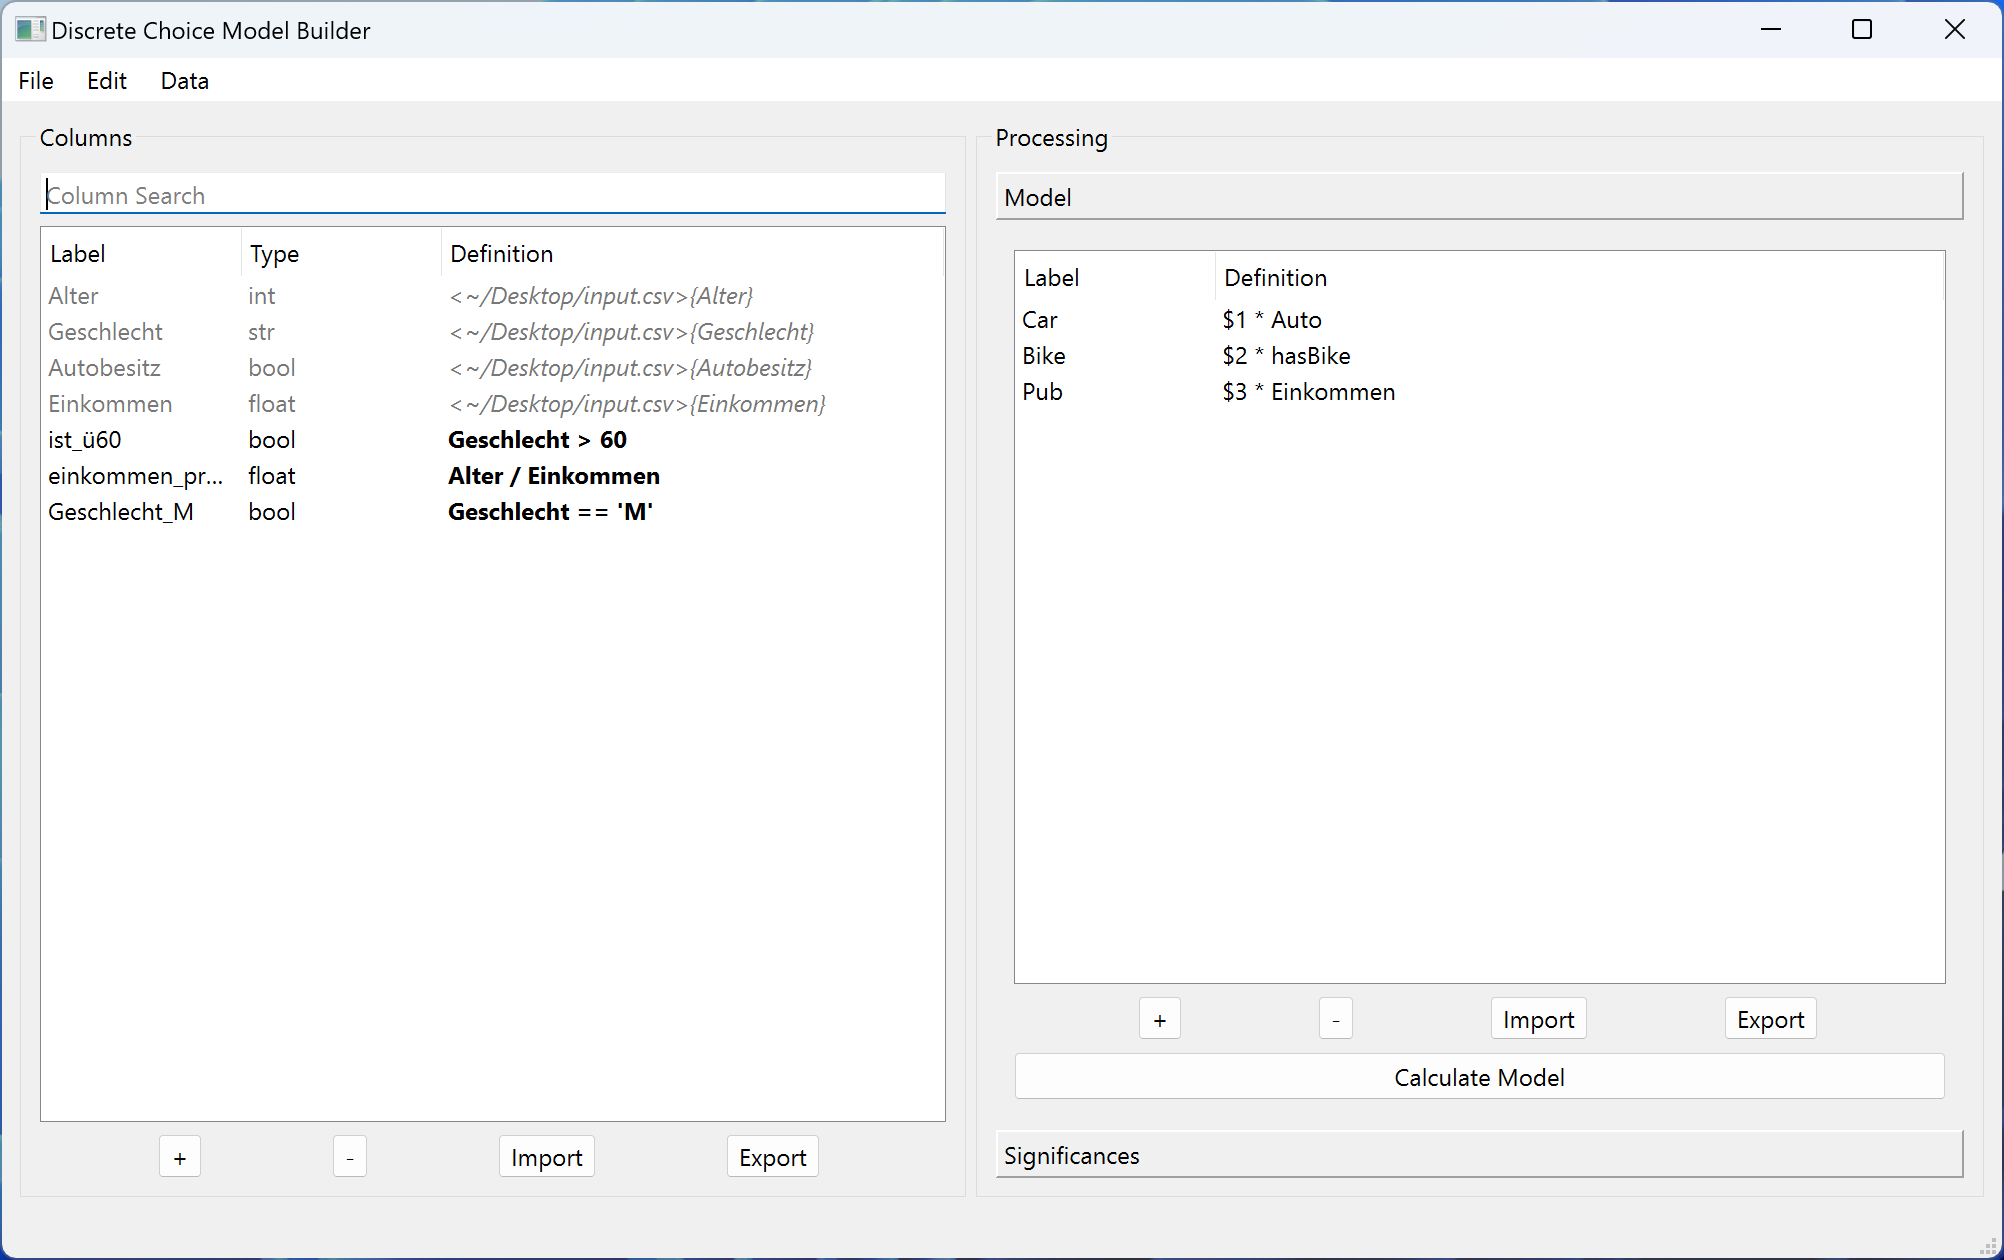
\includegraphics[width=12cm]{specifications/img/gui-screenshots/columns+model.png}
  \caption{GUI Entwurf}
\end{figure}

\clearpage
\section{Globale Testfälle}

\subsection{Funktionssequenzen}
Folgende Funktionen sind zu überprüfen.

\begin{table}[H]
\begin{tabularx}{\textwidth}{rX}
\vspace{1mm}
\textbf{/T10/}         & \textbf{Importieren der CSV-Datei} \\ \vspace{1mm}
\textbf{Produktfunktion} & \textbf{/F10/} \\ \vspace{1mm}
\textbf{Vorbedingung}  & Das Programm ist gestartet. \\ \vspace{1mm}
\textbf{Beschreibung}  & Der Nutzer wählt die CSV-Datei aus. \\
\textbf{Nachbedingung} & Die CSV-Datei wurde importiert und die enthaltenen Werte wurden in das Programm eingelesen.
\end{tabularx}
\end{table}

\begin{table}[H]
\begin{tabularx}{\textwidth}{rX}
 \vspace{1mm}
\textbf{/T20/}         & \textbf{Exportieren der CSV-Datei (Erfolg)} \\ \vspace{1mm}
\textbf{Produktfunktion} & \textbf{/F13/} \\
\textbf{Vorbedingung}  & Die CSV-Datei ist im Programm geladen. \\ \vspace{1mm} & Alle Attributsableitungen sind valide. \\ \vspace{1mm}
\textbf{Beschreibung}  & Der Nutzer exportiert die CSV-Datei. \\
\textbf{Nachbedingung} & Es wurde eine neue CSV-Datei mit allen Attributsableitungen erstellt.
\end{tabularx}
\end{table}

\begin{table}[H]
\begin{tabularx}{\textwidth}{rX}
 \vspace{1mm}
\textbf{/T21/}         & \textbf{Exportieren der CSV-Datei (Teilerfolg)} \\ \vspace{1mm}
\textbf{Produktfunktion} & \textbf{/F13/} \\
\textbf{Vorbedingung}  & Die CSV-Datei ist im Programm geladen. \\ \vspace{1mm} & Es existieren invalide Attributsableitungen. \\
\textbf{Beschreibung}  & Der Nutzer exportiert die CSV-Datei. \\ & Das Programm meldet invalide Attributsableitungen. \\ \vspace{1mm} & Der Nutzer führt den Export fort. \\
\textbf{Nachbedingung} & Es wurde eine neue CSV-Datei mit allen validen Attributsableitungen erstellt.
\end{tabularx}
\end{table}

\begin{table}[H]
\begin{tabularx}{\textwidth}{rX}
 \vspace{1mm}
\textbf{/T22/}         & \textbf{Exportieren der CSV-Datei (Abbruch)} \\ \vspace{1mm}
\textbf{Produktfunktion} & \textbf{/F13/} \\
\textbf{Vorbedingung}  & Die CSV-Datei ist im Programm geladen. \\  \vspace{1mm}& Es existieren invalide Attributsableitungen. \\
\textbf{Beschreibung}  & Der Nutzer exportiert die CSV-Datei. \\ & Das Programm meldet invalide Attributsableitungen. \\ \vspace{1mm} & Der Nutzer bricht den Export ab. \\
\textbf{Nachbedingung} & Der Zustand des Programms bleibt unverändert.
\end{tabularx}
\end{table}

\begin{table}[H]
\begin{tabularx}{\textwidth}{rX}
 \vspace{1mm}
\textbf{/T30/}         & \textbf{Projekt laden} \\ \vspace{1mm}
\textbf{Produktfunktion} & \textbf{/F11/} \\ \vspace{1mm}
\textbf{Vorbedingung}  & Das Programm ist gestartet.   \\ \vspace{1mm}
\textbf{Beschreibung}  & Der Nutzer wählt die Projektdatei aus. \\
\textbf{Nachbedingung} & Das Projekt wurde geladen.
\end{tabularx}
\end{table}

\begin{table}[H]
\begin{tabularx}{\textwidth}{rX}
 \vspace{1mm}
\textbf{/T31/}         & \textbf{Projekt speichern (Erfolg)} \\ \vspace{1mm}
\textbf{Produktfunktion} & \textbf{/F12/} \\
\textbf{Vorbedingung}  & Das Projekt ist geöffnet.   \\ \vspace{1mm} & Alle Eingaben sind valide. \\ \vspace{1mm}
\textbf{Beschreibung}  & Der Nutzer speichert das Projekt. \\
\textbf{Nachbedingung} & Das Projekt wurde gespeichert.
\end{tabularx}
\end{table}

\begin{table}[H]
\begin{tabularx}{\textwidth}{rX}
 \vspace{1mm}
\textbf{/T32/}         & \textbf{Projekt speichern (Erfolg)} \\ \vspace{1mm}
\textbf{Produktfunktion} & \textbf{/F12/} \\
\textbf{Vorbedingung}  & Das Projekt ist geöffnet.   \\ \vspace{1mm} & Es existieren invalide Eingaben. \\
\textbf{Beschreibung}  & Der Nutzer speichert das Projekt. \\ & Das Programm meldet invalide Eingaben. \\ \vspace{1mm} & Der Nutzer führt das Speichern fort. \\
\textbf{Nachbedingung} & Das Projekt wurde gespeichert.
\end{tabularx}
\end{table}

\begin{table}[H]
\begin{tabularx}{\textwidth}{rX}
 \vspace{1mm}
\textbf{/T33/}         & \textbf{Projekt speichern (Abbruch)} \\ \vspace{1mm}
\textbf{Produktfunktion} & \textbf{/F12/} \\
\textbf{Vorbedingung}  & Das Projekt ist geöffnet.   \\ \vspace{1mm} & Es existieren invalide Eingaben. \\
\textbf{Beschreibung}  & Der Nutzer speichert das Projekt. \\ & Das Programm meldet invalide Eingaben. \\ \vspace{1mm} & Der Nutzer bricht das Speichern ab. \\
\textbf{Nachbedingung} & Es wurde keine Speicherung vorgenommen.  
\end{tabularx}
\end{table}

\begin{table}[H]
\begin{tabularx}{\textwidth}{rX}
 \vspace{1mm}
\textbf{/T40/}         & \textbf{Attributsableitung hinzufügen (Erfolg)} \\ \vspace{1mm}
\textbf{Produktfunktion} & \textbf{/F15/} \\ \vspace{1mm}
\textbf{Vorbedingung}  & Die CSV-Datei wurde vollständig geladen.   \\ \vspace{1mm}
\textbf{Beschreibung}  & Der Nutzer gibt eine valide Attributsableitung ein und fügt sie hinzu. \\
\textbf{Nachbedingung} & Die Attributsableitung wird hinzugefügt.\\
\end{tabularx}
\end{table}

\begin{table}[H]
\begin{tabularx}{\textwidth}{rX}
 \vspace{1mm}
\textbf{/T41/}         & \textbf{Attributsableitung hinzufügen (Misserfolg)} \\ \vspace{1mm}
\textbf{Produktfunktion} & \textbf{/15/} \\ \vspace{1mm}
\textbf{Vorbedingung}  & Die CSV-Datei wurde vollständig geladen.   \\ \vspace{1mm}
\textbf{Beschreibung}  & Der Nutzer gibt eine invalide Attributsableitung ein und fügt sie hinzu. \\
\textbf{Nachbedingung} & Die Attributsableitung wird nicht hinzugefügt. \\ & Der Nutzer erhält eine Fehlermeldung, welche auf den Fehler hinweist.
\end{tabularx}
\end{table}

\begin{table}[H]
\begin{tabularx}{\textwidth}{rX}
 \vspace{1mm}
\textbf{/T42/}         & \textbf{Attributsableitung ändern (Erfolg)} \\ \vspace{1mm}
\textbf{Produktfunktion} & \textbf{/16/} \\
\textbf{Vorbedingung}  & Die CSV-Datei wurde vollständig geladen. \\ \vspace{1mm} & Es existiert mindestens eine Attributsableitung.  \\ \vspace{1mm}
\textbf{Beschreibung}  & Der Nutzer wählt eine Attributsableitung aus, gibt eine valide Attributsableitung ein und wendet die Änderung an. \\
\textbf{Nachbedingung} & Die ausgewählte Attributsableitung wird geändert.
\end{tabularx}
\end{table}

\begin{table}[H]
\begin{tabularx}{\textwidth}{rX}
 \vspace{1mm}
\textbf{/T43/}         & \textbf{Attributsableitung ändern (Misserfolg)} \\ \vspace{1mm}
\textbf{Produktfunktion} & \textbf{/16/} \\
\textbf{Vorbedingung}  & Die CSV-Datei wurde vollständig geladen. \\ \vspace{1mm} & Es existiert mindestens eine Attributsableitung.   \\ \vspace{1mm}
\textbf{Beschreibung}  & Der Nutzer wählt eine Attributsableitung aus, gibt eine valide Attributsableitung ein und wendet die Änderung an. \\
\textbf{Nachbedingung} & Die ausgewählte Attributsableitung wird nicht geändert. \\ & Der Nutzer erhält eine Fehlermeldung, welche auf den Fehler hinweist.
\end{tabularx}
\end{table}

\begin{table}[H]
\begin{tabularx}{\textwidth}{rX}
 \vspace{1mm}
\textbf{/T44/}         & \textbf{Attributsableitung löschen (Erfolg)} \\ \vspace{1mm}
\textbf{Produktfunktion} & \textbf{/17/} \\
\textbf{Vorbedingung}  & Die CSV-Datei wurde vollständig geladen. \\ & Es existiert mindestens eine Attributsableitung.  \\ \vspace{1mm} & Andere Eingaben haben eine Abhängigkeit zu der ausgewählten Attributsableitung. \\ \vspace{1mm}
\textbf{Beschreibung}  & Der Nutzer wählt eine Attributsableitung aus und löscht sie. \\
\textbf{Nachbedingung} & Die ausgewählte Attributsableitung wird gelöscht.
\end{tabularx}
\end{table}

\begin{table}[H]
\begin{tabularx}{\textwidth}{rX}
 \vspace{1mm}
\textbf{/T45/}         & \textbf{Attributsableitung löschen (Erfolg)} \\ \vspace{1mm}
\textbf{Produktfunktion} & \textbf{/17/} \\
\textbf{Vorbedingung}  & Die CSV-Datei wurde vollständig geladen. \\ & Es existiert mindestens eine Attributsableitung.  \\ \vspace{1mm} & Andere Eingaben haben eine Abhängigkeit zu der ausgewählten Attributsableitung. \\
\textbf{Beschreibung}  & Der Nutzer wählt eine Attributsableitung aus und löscht sie. \\ & Das Programm meldet eine Abhängigkeit zu dieser Ableitung. \\ \vspace{1mm} & Der Nutzer führt das Löschen fort. \\
\textbf{Nachbedingung} & Die ausgewählte Attributsableitung wird gelöscht. \\ & Die abhängigen Eingaben werden als invalide markiert.
\end{tabularx}
\end{table}

\begin{table}[H]
\begin{tabularx}{\textwidth}{rX}
 \vspace{1mm}
\textbf{/T46/}         & \textbf{Attributsableitung löschen (Abbruch)} \\ \vspace{1mm}
\textbf{Produktfunktion} & \textbf{/17/} \\
\textbf{Vorbedingung}  & Die CSV-Datei wurde vollständig geladen. \\ & Es existiert mindestens eine Attributsableitung.  \\ \vspace{1mm} & Andere Eingaben haben eine Abhängigkeit zu der ausgewählten Attrbiutsableitung. \\
\textbf{Beschreibung}  & Der Nutzer wählt eine Attributsableitung aus und löscht sie. \\ & Das Programm meldet eine Abhängigkeit zu dieser Ableitung. \\ \vspace{1mm} & Der Nutzer bricht den Löschvorgang ab. \\
\textbf{Nachbedingung} & Der Zustand des Programms bleibt unverändert.
\end{tabularx}
\end{table}
\textbf{Mögliche weitere Testfälle}
\begin{itemize}
    \item (?) Meldung über Abhängigkeit in anderer Ableitung, alle abhängigen Ableitungen löschen
\end{itemize}

\begin{table}[H]
\begin{tabularx}{\textwidth}{rX}
 \vspace{1mm}
\textbf{/T50/}         & \textbf{Alternative hinzufügen (Erfolg)} \\ \vspace{1mm}
\textbf{Produktfunktion} & \textbf{/20/} \\ \vspace{1mm}
\textbf{Vorbedingung}  & Die CSV-Datei wurde vollständig geladen.   \\ \vspace{1mm}
\textbf{Beschreibung}  & Der Nutzer gibt eine valide Alternative ein und fügt sie hinzu. \\
\textbf{Nachbedingung} & Die Alternative wurde hinzugefügt.
\end{tabularx}
\end{table}

\begin{table}[H]
\begin{tabularx}{\textwidth}{rX}
 \vspace{1mm}
\textbf{/T51/}         & \textbf{Alternative hinzufügen (Misserfolg)} \\ \vspace{1mm}
\textbf{Produktfunktion} & \textbf{/20/} \\ \vspace{1mm}
\textbf{Vorbedingung}  & Die CSV-Datei wurde vollständig geladen.   \\ \vspace{1mm}
\textbf{Beschreibung}  & Der Nutzer gibt eine Alternative mit invalider Nutzenfunktion oder bereits existierendem Namen ein und fügt sie hinzu. \\
\textbf{Nachbedingung} & Die Alternative wird nicht hinzugefügt. \\ & Der Nutzer erhält eine Fehlermeldung, welche auf den Fehler hinweist.
\end{tabularx}
\end{table}

\begin{table}[H]
\begin{tabularx}{\textwidth}{rX}
 \vspace{1mm}
\textbf{/T52/}         & \textbf{Alternative ändern (Erfolg)} \\ \vspace{1mm}
\textbf{Produktfunktion} & \textbf{/21/} \\ \vspace{1mm}
\textbf{Vorbedingung}  & Die CSV-Datei wurde vollständig geladen. Es existiert mindestens eine Alternative.  \\ \vspace{1mm}
\textbf{Beschreibung}  & Der Nutzer wählt eine Alternative aus, gibt eine valide Alternative ein und wendet die Änderung an. \\
\textbf{Nachbedingung} & Die ausgewählte Alternative wird geändert.
\end{tabularx}
\end{table}

\begin{table}[H]
\begin{tabularx}{\textwidth}{rX}
 \vspace{1mm}
\textbf{/T53/}         & \textbf{Alternative ändern (Misserfolg)} \\ \vspace{1mm}
\textbf{Produktfunktion} & \textbf{/21/} \\ \vspace{1mm}
\textbf{Vorbedingung}  & Die CSV-Datei wurde vollständig geladen. Es existiert mindestens eine Alternative.   \\ \vspace{1mm}
\textbf{Beschreibung}  & Der Nutzer wählt eine Alternative aus, gibt eine Alternative mit invalider Nutzenfunktion oder bereits existierendem Namen ein und wendet die Änderung an. \\
\textbf{Nachbedingung} & Die ausgewählte Nutzenfunktion wird nicht geändert. \\ & Der Nutzer erhält eine Fehlermeldung, welche auf den Fehler hinweist.
\end{tabularx}
\end{table}

\begin{table}[H]
\begin{tabularx}{\textwidth}{rX}
 \vspace{1mm}
\textbf{/T54/}         & \textbf{Alternative löschen} \\ \vspace{1mm}
\textbf{Produktfunktion} & \textbf{/22/} \\ \vspace{1mm}
\textbf{Vorbedingung}  & Die CSV-Datei wurde vollständig geladen. Es existiert mindestens eine Alternative.  \\ \vspace{1mm}
\textbf{Beschreibung}  & Der Nutzer wählt eine Alternative aus und löscht diese. \\
\textbf{Nachbedingung} & Die ausgewählte Alternative wird gelöscht.
\end{tabularx}
\end{table}


%begin{table}[H]
%\begin{tabularx}{\textwidth}{rX}
%\textbf{/T55/}         & \textbf{Linearkombination von Nutzenfunktionen anwenden} \\
%\textbf{Vorbedingung}  & Die CSV-Datei wurde vollständig geladen. Es existiert %mindestens eine Nutzenfunktion.  \\
%\textbf{Beschreibung}  & Der Nutzer wählt mindestens eine Nutzenfunktion aus und %erstellt eine Linearkombination. (MK4.1) \\
%\textbf{Nachbedingung} & Die konfigurierte Linearkombination der Nutzenfunktionen wird %berechnet.
%\end{tabularx}
%\end{table}


\begin{table}[H]
\begin{tabularx}{\textwidth}{rX} \vspace{1mm}
\textbf{/T60/}         & \textbf{Berechnung durchführen (Erfolg)} \\ \vspace{1mm}
\textbf{Produktfunktion} & \textbf{/25/} \\
\textbf{Vorbedingung}  & Die CSV-Datei wurde vollständig geladen. \\ & Es existiert mindestens eine Alternative. \\ \vspace{1mm} & Alle Alternativen sind valide. \\ \vspace{1mm}
\textbf{Beschreibung}  & Der Nutzer führt die Berechnung durch. \\
\textbf{Nachbedingung} & Die Parameter und Signifikanzen aller Alternativen wurden berechnet.
\end{tabularx}
\end{table}

\begin{table}[H]
\begin{tabularx}{\textwidth}{rX} \vspace{1mm}
\textbf{/T61/}         & \textbf{Berechnung durchführen (Erfolg)} \\ \vspace{1mm}
\textbf{Produktfunktion} & \textbf{/25/} \\
\textbf{Vorbedingung}  & Die CSV-Datei wurde vollständig geladen. \\ & Es existiert mindestens eine Alternative. \\ \vspace{1mm} & Es existieren invalide Alternativen. \\
\textbf{Beschreibung}  & Der Nutzer führt die Berechnung durch. \\ & Das Programm meldet invalide Alternativen. \\ \vspace{1mm} & Der Nutzer führt die Berechnung fort. \\
\textbf{Nachbedingung} & Die Parameter und Signifikanzen der validen Alternativen wurden berechnet.
\end{tabularx}
\end{table}

\begin{table}[H]
\begin{tabularx}{\textwidth}{rX} \vspace{1mm}
\textbf{/T62/}         & \textbf{Berechnung durchführen (Abbruch)} \\ \vspace{1mm}
\textbf{Produktfunktion} & \textbf{/25/} \\
\textbf{Vorbedingung}  & Die CSV-Datei wurde vollständig geladen. \\ & Es existiert mindestens eine Alternative. \\ \vspace{1mm} & Es existieren invalide Alternativen. \\
\textbf{Beschreibung}  & Der Nutzer führt die Berechnung durch. \\ & Das Programm meldet invalide Alternativen. \\ \vspace{1mm} & Der Nutzer bricht die Berechnung ab. \\
\textbf{Nachbedingung} & Der Zustand des Programms bleibt unverändert.
\end{tabularx}
\end{table}

\begin{table}[H]
\begin{tabularx}{\textwidth}{rX} \vspace{1mm}
\textbf{/T63/}         & \textbf{Berechnung durchführen (Abbruch)} \\ \vspace{1mm}
\textbf{Produktfunktion} & \textbf{/25/} \\
\textbf{Vorbedingung}  & Die CSV-Datei wurde vollständig geladen. \\ \vspace{1mm} & Es existiert mindestens eine Alternative. \\
\textbf{Beschreibung}  & Der Nutzer führt die Berechnung durch. \\ \vspace{1mm} & Der Nutzer bricht die Berechnung mittendrin ab. \\
\textbf{Nachbedingung} & Der Zustand des Programms bleibt unverändert.
\end{tabularx}
\end{table}

\begin{table}[H]
\begin{tabularx}{\textwidth}{rX} \vspace{1mm}
\textbf{/70/}         & \textbf{Exportieren der Ergebnisse}  \\ \vspace{1mm}
\textbf{Produktfunktion} & \textbf{/F28/} \\
\textbf{Vorbedingung}  & Die CSV-Datei ist im Programm geladen. \\ \vspace{1mm} & Die Berechnungen sind abgeschlossen.   \\ \vspace{1mm}
\textbf{Beschreibung}  & Der Nutzer exportiert die berechneten Ergebnisse. \\
\textbf{Nachbedingung} & Es wurde eine neue CSV-Datei erstellt, die die berechneten Ergebnisse enthält.
\end{tabularx}
\end{table}

\begin{table}[H]
\begin{tabularx}{\textwidth}{rX} \vspace{1mm}
\textbf{/T75/}         & \textbf{Änderung der Schwellwerte} \\ \vspace{1mm}
\textbf{Produktfunktion} & \textbf{/F30/} \\
\textbf{Vorbedingung}  & Die CSV-Datei wurde geladen. \\ & Die Berechnungen sind abgeschlossen. \\ \vspace{1mm} & Die Visualisierung der Ergebnisse wird angezeigt.\\ \vspace{1mm}
\textbf{Beschreibung}  & Der Nutzer ändert den Schwellwert. \\
\textbf{Nachbedingung} & Die Änderung des Schwellwerts wurde übernommen. \\ & Die Visualisierung wird reevaluiert.
\end{tabularx}
\end{table}


\subsection{Datenkonsistenzen}
Folgende Datenkonsistenzen sind einzuhalten.
\begin{table}[H]
\begin{tabularx}{\textwidth}{rX}
\textbf{/T1000/}        & Rohdaten werden unverändert gespeichert. \\              \textbf{/T1001/}        & Das Einlesen einer gespeicherten CSV-Datei resultiert im gleichen Programmzustand wie vor dem Speichervorgang.? \\
\end{tabularx}
\end{table}

\clearpage
\section{Qualitätsbestimmung}
\subsection{Funktionalität}
\begin{table}[H]
\centering
\begin{tabular}{lcccc}
\hline
\textbf{Produktqualität} & sehr gut & gut & normal & nicht relevant \\ \hline
Angemessenheit           &          &     & X      &                \\
Richtigkeit              & X        &     &        &                \\
Interoperabilität        &          & X   &        &                \\
Ordnungsmäßigkeit        &          &     &        & X              \\
Sicherheit               &          &     &        & X              \\  
\end{tabular}
\end{table}
Die Richtigkeit der Berechnungen nimmt höchsten Stellenwert an. Auch die Interoperabilität, insbesondere die Interaktion mit Biogeme zur Berechnung der Discrete Choice Modelle, ist wichtig. Weder Ordnungsmäßigkeit noch Sicherheit spielen eine Rolle in der Funktionalität.

\subsection{Zuverlässigkeit}
\begin{table}[H]
\centering
\begin{tabular}{lcccc}
\hline
\textbf{Produktqualität} & sehr gut & gut & normal & nicht relevant \\ \hline
Reife                    &          &     & X      &                \\
Fehlertoleranz           & X        &     &        &                \\
Wiederherstellbarkeit    &          & X   &        &                \\
\end{tabular}
\end{table}
Die Fehlertoleranz nimmt hohen Stellenwert ein um Einschränkungen an den Nutzer gering zu halten. Durch gesicherte Wiederherstellbarkeit der Projektabläufe ist Zuverlässigkeit des Programmes gegeben. 

\subsection{Benutzbarkeit}
\begin{table}[H]
\centering
\begin{tabular}{lcccc}
\hline
\textbf{Produktqualität} & sehr gut & gut & normal & nicht relevant \\ \hline
Verständlichkeit         &          & X   &        &                \\
Erlernbarkeit            &          & X   &        &                \\
Bedienbarkeit            & X        &     &        &                \\
\end{tabular}
\end{table}
Es wird besonders Wert gelegt auf die Benutzbarkeit des Baukastens durch eine sehr gute Bedienbarkeit. Das Programm soll einfach in der Anwendung sein durch seinen verständlichen und erlernbaren Ablauf.

\subsection{Effizienz}
\begin{table}[H]
\centering
\begin{tabular}{lcccc}
\hline
\textbf{Produktqualität} & sehr gut & gut & normal & nicht relevant \\ \hline
Zeitverhalten            &          &     & X      &                \\
Verbrauchsverhalten      &          &     & X      &               
\end{tabular}
\end{table}
Die Effizienz sowohl in der Zeit als auch im Speicherbedarf nimmt keinen hohen Stellenwert an. 

\subsection{Änderbarkeit}
\begin{table}[H]
\centering
\begin{tabular}{lcccc}
\hline
\textbf{Produktqualität} & sehr gut & gut & normal & nicht relevant \\ \hline
Analysierbarkeit         &          & X   &        &                \\
Modifizierbarkeit        & X        &     &        &                \\
Stabilität               & X        &     &        &                \\
Prüfbarkeit              & X        &     &        &                \\
\end{tabular}
\end{table}
Die Änderbarkeit des Programms ist von höchster Bedeutung. Das Programm soll modifizierbar sein, um verschiedene Bibliotheken zur Berechnung von Discrete Choice Modellen zu unterstützen, und die Einbindung von Algorithmen zur Erweiterbarkeit erlauben.

\newpage
% AAAHHH WARUM FUNKTIONIERT DAS NICHT?
% Den gleichen Code in ein neues Dokument kopieren lässt das Glossar wieder erscheinen - aber den Cache leeren ändert hier nichts
\printglossaries

\end{document}